\documentclass[12pt,a4paper]{report}
\usepackage{graphicx}
\usepackage{setspace}
\usepackage{geometry}
\usepackage{amsmath}
\usepackage{amsfonts}
\usepackage{amssymb}
\usepackage{titlesec}
\usepackage{lipsum}
\usepackage{url}

% Setting margins
% \usepackage[left=1.5in, right=1in, top=1.5in, bottom=1in, includefoot, includehead]{geometry}

\geometry{
    % Odd numbered pages
    inner=1in, % Left margin for odd numbered pages
    outer=1.5in, % Right margin for odd numbered pages
    top=1.5in,
    bottom=1in,
    % Even numbered pages
    twoside,
    left=1.5in, % Left margin for even numbered pages
    right=1in % Right margin for even numbered pages
}




% Chapter formatting
\titleformat{\chapter}[hang]
  {\normalfont\bfseries}{\chaptertitlename\ \thechapter}{20pt}{\MakeUppercase}

% Use Times New Roman font
\usepackage{times}


% Set spacing to 1.5
\onehalfspacing

%Customizing chapter and section headings
% \titleformat{\chapter}[hang]{\bfseries\fontsize{12}{14}\selectfont}{\thechapter\hspace{12pt}}{0pt}{\bfseries\MakeUppercase}
% \titlespacing*{\chapter}{0pt}{0pt}{20pt}
% \titleformat{\section}[hang]{\bfseries\fontsize{12}{14}\selectfont}{\thesection\hspace{12pt}}{0pt}{\bfseries\MakeUppercase}
% \titlespacing*{\section}{0pt}{20pt}{10pt}
% \titleformat{\subsection}[hang]{\fontsize{12}{14}\selectfont}{\thesubsection\hspace{12pt}}{0pt}{}

% Define chapter format
\titleformat{\chapter}[hang]
  {\normalfont\fontsize{14}{16}\bfseries}{\MakeUppercase{\chaptertitlename}\ \thechapter}{20pt}{\MakeUppercase}

% Define section and subsection format
\titleformat{\section}
  {\normalfont\fontsize{12}{14}\bfseries}{\thesection}{1em}{\MakeUppercase}
\titleformat{\subsection}
  {\normalfont\fontsize{12}{14}\bfseries}{\thesubsection}{1em}{}


% Beginning of the document
\begin{document}

% Title Page
\begin{titlepage}
    \centering
    % Title
    {\Huge \bfseries{RECONCILIATION FLOW CONTROL}\par}
    \vspace{0.5cm}
    {\large Thesis\\ \par}
    {\large Submitted in partial fulfilment of the requirements for the degree of\par}
  \vspace{0.5cm}
    {\Large\bfseries MASTER OF COMPUTER APPLICATIONS\par}  % Uncomment this for MCA
    % {\Large\bfseries Master of Science\par}   % Uncomment this for M.Sc.
  \vspace{0.5cm}
    {\large by\par}
  \vspace{0.5cm}
    {\Large\bfseries UTKARSH AGARWAL\par}
    \vspace{0.5cm}
    {\Large\bfseries (2140046)\par}
  \vspace{0.5cm}
    % University Logo
    
\includegraphics[width=0.4\textwidth]{images/NITK_Emblem.png}\\
    \vspace{1cm}
    % Department and University
    {\large\bfseries DEPARTMENT OF MATHEMATICAL AND COMPUTATIONAL SCIENCES \par} 
    \vspace{0.5cm}
    {\large\bfseries NATIONAL INSTITUTE OF TECHNOLOGY KARNATAKA \par} 
    {\large\bfseries SURATHKAL, MANGALORE - 575025\par}
    \vspace{0.5cm}
    {\large\bfseries JUNE, 2024\par}
\end{titlepage}

\pagenumbering{roman}
% Declaration Page
\chapter*{Declaration}
I hereby declare that the Project Report entitled \textbf{“Reconciliation FLow Control”} which is being submitted to the \textbf{National Institute of Technology Karnataka, Surathkal}, in partial fulfillment of the requirements for the degree of \textbf{Master of Computer Applications} in the \textbf{Department of Mathematical and Computational Sciences}, is a bonafide report of the work carried out by me.

\vspace{1cm}

\begin{flushright}
UTKARSH AGARWAL \\
2140046CA061
\end{flushright}


% Certificate Page
\chapter*{Certificate}
% Certificate content here

% Acknowledgement Page
\chapter*{Acknowledgement}

The satisfaction that is generated by the successful completion of a task would remain unfulfilled without mentioning people who have encouraged and guided me at every step towards the completion of the task. Starting with, I would like to extend my sincere thanks to my guide in the company, \textbf{Mr. Anish Kurian, Senior Engineering Manager at Zeta}, for giving me the opportunity to work under him. This opportunity gave me a chance to sharpen my working methodology to a higher extent and to solve the problems in a better and easy way, so that it can be presented in a better and understandable manner. My heartfelt gratitude also goes to Professor \textbf{Dr. P. Sam Johnson}, Head of the Department, Department of Mathematical and Computational Sciences, National Institute of Technology Karnataka, Surathkal, for providing me with the opportunity to avail the excellent facilities and infrastructure of the institute.
\\\\
\noindent I would also like to thank my mentor, Associate Professor \textbf{Dr. Vivek Sinha}, Department of Mathematical and Computational Sciences, National Institute of Technology Karnataka, Surathkal, for his continuous guidance and support. The knowledge and values inculcated have proved to be of immense help.
\\\\
\noindent I am very thankful to \textbf{Zeta}, for giving me the opportunity to work under their experienced team. This would never be complete without thanking my parents and my family for their constant support and encouragement and of course my friends and teammates for helping me throughout the process.

\vspace{1cm}

\begin{flushright}
UTKARSH AGARWAL \\
2140046CA0061
\end{flushright}

% Acknowledgement content here

% Abstract Page
\chapter*{Abstract}
This thesis explores the development and optimization of a high-traffic API system for financial transactions, focusing on enhancing performance, scalability, and reliability. The project began with an extensive Knowledge Acquisition phase, aimed at understanding domain-specific challenges and relevant technologies such as Kafka, Spring Boot, Grafana, Kibana, and Jenkins. This foundational knowledge was crucial for informed decision-making and successful implementation.
\\\\
\noindent The core of the project involved backend development, where key activities included setup and configuration, database design, API development, business logic implementation, and rigorous testing. Security measures were implemented using Spring Security to ensure robust authentication and authorization. Integration testing and the use of Retrofit for external API communication ensured seamless interaction between backend components, enhancing overall system reliability.
\\\\
\noindent Deployment and documentation were meticulously planned, utilizing CI/CD pipelines, Kubernetes, and AWS for scalable and reliable environments. Comprehensive documentation was provided to support users and administrators. The project concluded with a systematic bug-fixing process and continuous monitoring, ensuring long-term stability and performance. This project demonstrates the effectiveness of a collaborative and iterative approach in optimizing high-traffic API systems, laying a solid foundation for future advancements.

\section*{KEYWORDS} Backend Development, Java, Spring Boot, PostgreSQL, RESTful API, Kafka, Event Streaming, Asynchronous Processing, Performance Optimization, Continuous Integration and Deployment.

% Table of Contents
\tableofcontents



% List of Figures
% \listoffigures % Uncomment if you have figures

% List of Tables
% \listoftables % Uncomment if you have tables

% Nomenclature
% \chapter*{Nomenclature}
% Nomenclature content here


%apply main geometry
\restoregeometry

% CHAPTER 1: INTRODUCTION
\chapter{Introduction}
\pagenumbering{arabic} % Start page numbering from Chapter 1
This project has been undertaken at Zeta Suites (Better World Technology) and is oriented to cover my final semester project requirements. The documents aim to give an overview of the technical project executed during my internship. Subsequent chapters will help in understanding the problem statement and the work done in the project.

\section{About the Organization}
Zeta is a next-gen banking tech company founded in 2015 by Bhavin Turakhia and Ramki Gaddipati. The company provides credit and debit card issuer processing, BNPL, core banking, and mobile experiences. Zeta's products are offered to banks and fintechs.
\\\\
\noindent The company was founded in April 2015 by Bhavin Turakhia and Ramki Gaddipati. Initially, Zeta's offerings included employee tax benefits, automated cafeterias, employee gifting, and digital payments. In 2016, Bhavin Turakhia invested around \$19 million into Zeta. Initially, Zeta payments were only supported by the MasterCard network, but later the company also partnered with the National Payments Corporation of India's RuPay.
\\\\
\noindent In June 2017, the company invested 5-10 crore to buy a minority stake in an HR company called ZingHR. Zeta has partnerships with IDFC Bank, Sodexo, Excelity Global, Kotak Mahindra Bank, and RBL Bank. Zeta launched the first employee benefits survey in India along with Nielsen Holdings in April 2018. It also bought a minority stake in PeopleStrong in January 2018.
\\\\
\noindent In 2019, Zeta received an investment from Sodexo BRS at a valuation of \$300 million. In 2020, Zeta launched its technology platform-as-a-service in the Philippines and Vietnam, with Sodexo being its first client in these countries. In 2021, Zeta secured a Series C investment of \$250 million from SoftBank Vision Fund 2, valuing Zeta at \$1.45 billion. This is one of the largest single investments in a banking tech startup globally.
\\\\
\noindent At Zeta, the focus is on rethinking payments from core to the edge. From algorithms to form factors, applications to solutions, Zeta is led by the vision to make payments invisible and seamless. Zeta has built an Omni Stack for Financial Institutions (FIs) covering debit, credit, prepaid, loans, authentication, and Fraud and Risk Management (FRM).

% Add more content as needed...



\section{Software Development & Methodology}
\noindent The development of the web application, aimed at automating the creation of PayZapp follows a systematic approach grounded in industry best practices and principles of agile software development. The methodology emphasizes collaboration, iterative development, and responsiveness to changing requirements, enabling me to deliver a high-quality solution that meets the needs of the stakeholders effectively.

\subsection{Agile Development Methodology}
I have adopted an agile development methodology to guide the project from inception to delivery. Agile methodologies prioritize flexibility, adaptability, and customer collaboration, allowing me to respond quickly to feedback and deliver incremental value with each iteration. By breaking down the project into manageable increments, or sprints, we can maintain a steady pace of development while continuously refining and enhancing the product.

\subsection{Scrum Framework}
Within the agile paradigm, I employed the Scrum framework to structure the development process and facilitate effective teamwork. Scrum promotes transparency, inspection, and adaptation through defined roles, ceremonies, and artifacts, ensuring clear communication and alignment among team members. Key components of the Scrum framework include:

\begin{figure}[h]
  \centering
  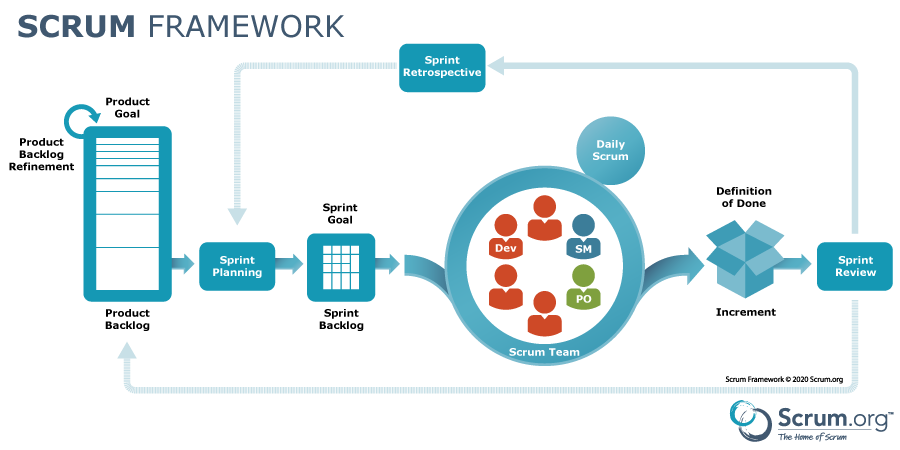
\includegraphics[width=5.5in]{images/scrum-framework-with-sdo-logo-9.29.23.png}\\[1.5cm]
  \caption{Scrum Flow}
  \label{fig:example}
\end{figure}



\begin{itemize}
    \item \textbf{Sprint Planning:} At the beginning of each sprint, the team collaboratively plans the work to be completed and commits to delivering a potentially shippable increment of functionality. 
    \item \textbf{Daily Stand-ups:} Daily stand-up meetings provide an opportunity for team members to synchronize their activities, discuss progress, and identify any impediments or blockers. 
    \item \textbf{Mid Sprint Check:} Ensuring we're on track with our sprint goals and identifying any blockers or adjustments needed.
    \item \textbf{Sprint Review:} At the end of each sprint, the team demonstrates the completed work to stakeholders and gathers feedback for future iterations. 
    \item \textbf{Sprint Retrospective:} A retrospective meeting allows the team to reflect on the previous sprint, identify areas for improvement, and adjust their processes accordingly.
\end{itemize}

\subsection{Iterative Development}
The project follows an iterative development approach, whereby functionality is incrementally developed, tested, and refined over multiple cycles. This iterative process allows to gather feedback early and often, validate assumptions, and make course corrections as needed. By delivering working software iteratively, I mitigated the risks associated with large-scale development efforts and ensure that the final product aligns closely with user needs and expectations.


\subsection{Continuous Integration and Deployment}
To streamline the development and release processes, I have implemented continuous integration and deployment practices. Through automation and integration with version control systems such as Git, we can automatically build, test, and deploy changes to our application in a consistent and reproducible manner. This enables to deliver updates to our users more frequently, with reduced risk and improved reliability.

 
% SECTION: PRODUCT OVERVIEW
\section{Product Overview}
PayZapp is a mobile wallet and online payment app offered by HDFC Bank in India. It acts as a versatile financial tool for users, enabling them to conduct a wide range of transactions conveniently and securely.

\subsection{Features and Functionalities}
\begin{itemize}
    \item \textbf{Payments:} PayZapp eliminates the need to juggle multiple payment methods. Users can handle a variety of transactions directly through the app, including bill payments for mobile recharge, DTH subscriptions, and utilities. Online shopping becomes a breeze, and in-store purchases are simplified with QR code scans at partner merchants. PayZapp even allows for easy money transfers to other PayZapp users or any bank account in India, offering a one-stop shop for all your financial needs.
    
    \item \textbf{Wallet and UPI Integration:} PayZapp functions as a prepaid wallet that can be loaded with funds for seamless transactions. Additionally, it integrates with the Unified Payments Interface (UPI) for instant money transfers and QR code-based payments.
    
    \item \textbf{Travel and Entertainment Bookings:} Users can book travel tickets (flights, trains, buses) and make hotel reservations directly through the app. Movie ticket bookings are also facilitated, and these bookings often come with cashback offers.
    
    \item \textbf{Security:} PayZapp prioritizes user safety with robust security features, including PIN and biometric authentication for logins, password protection for transactions, and no storage of card information on the user's device.
\end{itemize}

\subsection{Benefits of Using PayZapp}
\begin{itemize}
    \item \textbf{Convenience:} PayZapp simplifies financial management by offering a centralized platform for various transactions.
    \item \textbf{Security:} The app prioritizes user safety with advanced security measures.
    \item \textbf{Potential for Cashbacks and Discounts:} Users can benefit from cashback offers and discounts on transactions, including bill payments, shopping, and travel bookings.
\end{itemize}

\subsection{Target Audience}
PayZapp doesn't limit itself to a single user group. It strategically targets a diverse range of individuals and businesses in India:
\begin{itemize}
    \item \textbf{Tech-Savvy Urbanites:} Young, tech-comfortable Indians are a primary target. PayZapp's features align perfectly with their preference for online shopping, digital bill payments, and on-the-go convenience.
    \item \textbf{Existing HDFC Bank Customers:} As an HDFC Bank product, existing customers who trust and use the bank's digital services are a natural fit. Familiarity with the brand fosters quicker adoption of PayZapp.
    \item \textbf{Reaching the Unbanked:} India has a significant population without traditional bank accounts. PayZapp addresses this by potentially functioning without a linked bank account. Features like virtual accounts from HDFC can help them participate in the digital payments revolution.
    \item \textbf{Boosting Small Businesses:} While a separate "PayZapp for Business" service exists, the core app can still benefit small businesses. QR code payments allow them to receive payments from customers swiftly and conveniently.
\end{itemize}

\subsection{Overall Strategy}
This multi-pronged approach positions PayZapp to capture a significant share of the Indian mobile payments market. It caters to the growing tech-savvy population, offers financial inclusion to the unbanked, and provides solutions for small businesses.

\subsection{Availability}
The PayZapp app is readily available for download on the Google Play Store for Android devices and the Apple App Store for iOS devices.

\subsection{Additional Points to Consider}
\begin{itemize}
    \item \textbf{Competition:} The Indian mobile wallet market is competitive. You may want to mention PayZapp's competitors briefly in your report.
    \item \textbf{PayZapp for Business:} HDFC Bank offers a separate service called "PayZapp for Business" that allows businesses to receive payments from customers through the PayZapp platform.
\end{itemize}



% CHAPTER 2: TOOLS & TECHNOLOGIES USED
\chapter{Tools \& Technologies Used}

The development of the web application involves the utilization of a variety of cutting-edge technologies and frameworks aimed at delivering a robust, scalable, and user-friendly solution. Each technology plays a crucial role in different aspects of the application, from backend development and data management to frontend design and user interaction. Below, I provide an overview of the key technologies employed in the project:

\section{Java: The Core Programming Language}

Java forms the foundation of PayZapp's development. It's a general-purpose, object-oriented programming language renowned for its:

\begin{itemize}
    \item \textbf{Platform Independence:} "Write once, run anywhere." Java code can run on various operating systems without modifications, thanks to the Java Virtual Machine (JVM). This simplifies development and deployment across diverse environments.
    
    \item \textbf{Object-Oriented Design:} Java's object-oriented paradigm promotes code reusability, modularity, and maintainability. Complex functionalities can be encapsulated within objects, fostering efficient development and easier code management.
    
    \item \textbf{Strong Performance:} Java offers efficient memory management and just-in-time (JIT) compilation, leading to optimized performance and smooth user experience.
    
    \item \textbf{Large Developer Community:} A vast and active Java developer community provides extensive resources, libraries, and frameworks, accelerating development and troubleshooting.
\end{itemize}
\section{Spring: A Robust Development Framework}

Spring is a popular open-source framework for building enterprise Java applications. PayZapp utilizes Spring's features to simplify development and streamline various aspects of the application:

\begin{itemize}
    \item \textbf{Dependency Injection:} Spring promotes loose coupling between components by managing dependencies through dependency injection. This improves code testability, maintainability, and flexibility.
    
    \item \textbf{Aspect-Oriented Programming (AOP):} Spring supports AOP, enabling developers to implement cross-cutting concerns like logging, security, and transaction management without modifying core business logic.
    
    \item \textbf{MVC (Model-View-Controller) Architecture:} Spring encourages the separation of concerns by following the MVC architecture. This promotes code organization, easier maintenance, and better testability.
    
    \item \textbf{Spring Security:} Spring Security provides comprehensive security features to protect PayZapp from unauthorized access and vulnerabilities. Features like user authentication, authorization, and encryption ensure a secure environment for financial transactions.
\end{itemize}

By leveraging Spring's robust framework, PayZapp benefits from efficient development processes, improved code organization, and enhanced security measures.

\section{Spring Boot: Rapid Application Development}

Spring Boot is a lightweight framework built on top of Spring that simplifies application development and deployment. PayZapp utilizes Spring Boot for its:

\begin{itemize}
    \item \textbf{Auto-configuration:} Spring Boot eliminates the need for extensive XML configuration files. It automatically configures many common dependencies and features, streamlining the development process.
    
    \item \textbf{Embedded Server:} Spring Boot applications can embed a server like Tomcat or Undertow within the application itself. This eliminates the need for a separate server installation, making deployment easier.
    
    \item \textbf{Starter Projects:} Spring Boot offers pre-configured starter projects for various functionalities like web development, data access, and security. These pre-built modules accelerate development by providing a foundation for common requirements.
\end{itemize}

Spring Boot's approach allows PayZapp to achieve faster development cycles, simpler deployments, and easier management of application dependencies.

\section{PostgreSQL: A Reliable Database Solution}

PostgreSQL serves as the primary database management system for PayZapp. This powerful open-source database offers:

\begin{itemize}
    \item \textbf{ACID Transactions:} PostgreSQL guarantees Atomicity, Consistency, Isolation, and Durability (ACID) for transactions, ensuring data integrity and consistency.
    
    \item \textbf{Scalability:} PostgreSQL can handle large datasets and high transaction volumes effectively, making it suitable for PayZapp's potential growth.
    
    \item \textbf{Object-Relational Features:} PostgreSQL supports object-relational features, allowing developers to map database tables to Java objects seamlessly. This simplifies data access and manipulation.
    
    \item \textbf{Open Source and Extensible:} Being open-source, PostgreSQL provides cost-effective database management and allows for customization through extensions.
\end{itemize}

PayZapp leverages PostgreSQL's reliability, scalability, and object-relational features to ensure secure and efficient storage and retrieval of user data and transaction information.

\section{Jenkins: Continuous Integration and Delivery}

Jenkins is an open-source automation server widely used for continuous integration and delivery (CI/CD) pipelines. PayZapp likely utilizes Jenkins for:

\begin{itemize}
    \item \textbf{Automated Builds:} Jenkins can automate the build process, including compiling code, running unit tests, and packaging the application.
    
    \item \textbf{Continuous Integration:} Jenkins facilitates continuous integration by automatically building and testing code changes upon every commit to the version control system.
    
    \item \textbf{Delivery Pipelines:} Jenkins allows for the creation of deployment pipelines that automate the process of deploying new versions of the application to different environments (development, testing, production).
\end{itemize}

Integrating Jenkins enables PayZapp to achieve faster development cycles, improved code quality, and efficient deployment workflows.

\section{Kafka: Real-time Data Streaming}

Apache Kafka is a distributed streaming platform that enables real-time data processing. PayZapp might leverage Kafka for:

\begin{itemize}
    \item \textbf{Microservices Communication:} Kafka can act as a central hub for communication between microservices within the PayZapp architecture. Microservices can publish and subscribe to relevant data streams through Kafka, facilitating efficient data exchange.
    
    \item \textbf{Real-time Transaction Processing:} Kafka allows for real-time processing of transaction data. This enables features like instant payment confirmations, fraud detection, and real-time analytics.
    
    \item \textbf{Scalability and Fault Tolerance:} Kafka is designed for scalability and fault tolerance. It can handle high volumes of data and recover from node failures, ensuring uninterrupted data flow.
\end{itemize}

By utilizing Kafka, PayZapp benefits from real-time data processing, efficient microservice communication, and a robust infrastructure for handling high-volume data streams.

\section{Kubernetes: Container Orchestration Platform}

Kubernetes is an open-source container orchestration platform that automates the deployment, scaling, and management of containerized applications. PayZapp leverages Kubernetes to streamline its application deployment and management processes, ensuring scalability, reliability, and portability across various environments.

\subsection{Key Features of Kubernetes}

\begin{itemize}
    \item \textbf{Container Orchestration:} Kubernetes provides automated container orchestration, allowing developers to deploy and manage containerized applications efficiently. It handles tasks such as scheduling, scaling, and load balancing, ensuring optimal resource utilization and application availability.
    
    \item \textbf{Service Discovery and Load Balancing:} Kubernetes offers built-in service discovery and load balancing mechanisms, enabling seamless communication between microservices and distributing traffic across multiple instances of an application for improved performance and reliability.
    
    \item \textbf{Self-Healing Capabilities:} Kubernetes monitors the health of applications and automatically restarts or replaces containers that fail. This self-healing capability helps maintain application availability and resilience in dynamic environments.
    
    \item \textbf{Declarative Configuration:} Kubernetes uses declarative configuration files to define the desired state of applications and infrastructure. This approach simplifies deployment and configuration management, making it easier to maintain consistency and repeatability.
    
    \item \textbf{Horizontal Scaling:} Kubernetes supports horizontal scaling of applications based on metrics such as CPU utilization or custom metrics. This enables applications to automatically scale up or down in response to changes in workload demand, ensuring efficient resource utilization and cost optimization.
\end{itemize}

\subsection{Use Cases in PayZapp}

In PayZapp, Kubernetes is employed for various purposes, including:

\begin{itemize}
    \item \textbf{Microservices Deployment:} Kubernetes is used to deploy and manage microservices-based architectures, allowing PayZapp to break down monolithic applications into smaller, more manageable components. This promotes agility, scalability, and independent development and deployment of services.
    
    \item \textbf{Continuous Delivery:} Kubernetes facilitates continuous delivery practices by automating the deployment pipeline and providing features such as rolling updates and canary deployments. This enables PayZapp to deliver new features and updates to production quickly and reliably.
    
    \item \textbf{Hybrid and Multi-Cloud Deployments:} Kubernetes provides a consistent platform for deploying and managing applications across hybrid and multi-cloud environments. PayZapp leverages Kubernetes to ensure portability and flexibility in its deployment strategies, enabling seamless migration and scaling across different cloud providers.
\end{itemize}

By leveraging Kubernetes, PayZapp enhances its ability to deploy, scale, and manage containerized applications effectively, driving agility, reliability, and innovation in its technology stack.

\section{Redis: A High-Performance In-Memory Data Store}

Redis is a versatile and high-performance in-memory data structure store that serves multiple purposes, including caching, database, and message broker functionalities. PayZapp leverages Redis for various aspects of its application architecture due to its speed, simplicity, and flexibility.

\subsection{Key Features of Redis}

Redis offers several key features that make it an attractive choice for PayZapp's infrastructure:

\begin{itemize}
    \item \textbf{In-Memory Data Storage:} Redis stores data primarily in RAM, allowing for extremely fast read and write operations. This makes it ideal for applications requiring low-latency data access.
    
    \item \textbf{Support for Multiple Data Structures:} Redis supports a wide range of data structures, including strings, lists, sets, hashes, and more. This versatility enables developers to model complex data requirements efficiently.
    
    \item \textbf{Persistence Options:} Redis provides different persistence options, including snapshotting and append-only file (AOF) persistence, to ensure data durability and fault tolerance.
    
    \item \textbf{Pub/Sub Messaging:} Redis implements a publish/subscribe messaging paradigm, allowing components of PayZapp to communicate asynchronously. This feature is particularly useful for real-time updates and event-driven architectures.
    
    \item \textbf{Built-in Replication:} Redis supports master-slave replication, enabling data redundancy and high availability. This ensures that PayZapp remains operational even in the event of node failures.
\end{itemize}

\subsection{Use Cases in PayZapp}

PayZapp employs Redis for various purposes across its infrastructure:

\begin{itemize}
    \item \textbf{Caching:} Redis acts as a caching layer to store frequently accessed data, such as user sessions, authentication tokens, and frequently queried database results. This reduces database load and improves application performance.
    
    \item \textbf{Session Management:} Redis is used to manage user sessions, storing session data in memory for quick retrieval and updates. This ensures seamless user experiences across different parts of the application.
    
    \item \textbf{Queueing and Task Management:} Redis's list data structure is utilized as a lightweight message queue for asynchronous task processing. Background jobs, such as email notifications and data processing tasks, are queued and processed efficiently.
    
    \item \textbf{Real-Time Analytics:} Redis's pub/sub functionality enables real-time analytics by allowing components to subscribe to data streams and process incoming events in real-time. This capability is crucial for monitoring and analyzing user activities and system performance.
\end{itemize}

\section{Kibana: Data Visualization and Exploration}

Kibana is an open-source data visualization platform commonly used with Elasticsearch, a search and analytics engine. While not directly interacting with data, PayZapp might integrate Kibana with Elasticsearch for:

\begin{itemize}
    \item \textbf{Log Analysis:} Kibana allows for visualizing and analyzing application logs. This helps developers identify errors, track system performance, and troubleshoot issues effectively.
    
    \item \textbf{Security Monitoring:} Security logs and event data can be visualized in Kibana, enabling security teams to monitor for suspicious activity and potential threats.
    
    \item \textbf{Real-time Dashboards:} Kibana can create real-time dashboards that display key metrics and data visualizations. These dashboards provide insights into system health, transaction status, and user behavior.
\end{itemize}

By leveraging Kibana alongside Elasticsearch, PayZapp gains valuable tools for data exploration, log analysis, security monitoring, and real-time visualization of key metrics.

\section{Elasticsearch: Distributed Search and Analytics Engine}

Elasticsearch is a distributed search and analytics engine designed for horizontal scalability, reliability, and real-time search capabilities. PayZapp utilizes Elasticsearch for various purposes within its application architecture, leveraging its powerful indexing and querying capabilities to store, search, and analyze large volumes of structured and unstructured data efficiently.

\subsection{Key Features of Elasticsearch}

\begin{itemize}
    \item \textbf{Full-Text Search:} Elasticsearch provides full-text search capabilities with support for complex queries, relevance scoring, and linguistic analysis. This allows PayZapp to deliver fast and accurate search results across a wide range of data types.
    
    \item \textbf{Distributed Architecture:} Elasticsearch is built on a distributed architecture, allowing data to be distributed across multiple nodes for horizontal scalability and fault tolerance. This ensures high availability and performance, even with large datasets and high query volumes.
    
    \item \textbf{Real-Time Data Ingestion:} Elasticsearch supports real-time data ingestion, enabling PayZapp to index and search data as soon as it becomes available. This is particularly useful for monitoring, log analysis, and real-time analytics applications.
    
    \item \textbf{Aggregation and Analytics:} Elasticsearch offers powerful aggregation capabilities for performing analytics on indexed data, including metrics, histograms, and aggregations. This enables PayZapp to derive insights from its data and make data-driven decisions.
    
    \item \textbf{Ecosystem Integration:} Elasticsearch integrates seamlessly with other components of the Elastic Stack, including Kibana for visualization and analysis, Logstash for data collection and processing, and Beats for lightweight data shippers. This cohesive ecosystem provides a comprehensive solution for data management and analytics.
\end{itemize}

\subsection{Use Cases in PayZapp}

In PayZapp, Elasticsearch is employed for various use cases, including:

\begin{itemize}
    \item \textbf{User Search and Personalization:} Elasticsearch powers the user search functionality in PayZapp, allowing users to search for products, services, or other users quickly and accurately. Elasticsearch's full-text search capabilities enable personalized search results based on user preferences and behavior.
    
    \item \textbf{Log and Event Analysis:} PayZapp utilizes Elasticsearch for log and event analysis, indexing and analyzing logs generated by various components of its infrastructure. Elasticsearch's real-time indexing and querying capabilities enable rapid troubleshooting, monitoring, and analysis of system logs and events.
    
    \item \textbf{Recommendation Engine:} Elasticsearch is used to power recommendation engines in PayZapp, providing personalized recommendations to users based on their browsing history, purchase behavior, and demographic information. Elasticsearch's aggregations and analytics capabilities facilitate the generation of relevant and timely recommendations.
\end{itemize}

By leveraging Elasticsearch, PayZapp enhances its search capabilities, accelerates data analysis, and delivers personalized experiences to its users, driving customer engagement and satisfaction.


\section{Grafana: Monitoring and Alerting}

Grafana is another open-source platform for data visualization and monitoring. PayZapp might utilize Grafana for:

\begin{itemize}
    \item \textbf{Real-time System Monitoring:} Grafana allows for creating dashboards that display real-time system metrics like CPU usage, memory consumption, and application response times. This provides insights into system health and performance bottlenecks.
    
    \item \textbf{Alerting:} Grafana can be configured to send alerts when certain thresholds are crossed, notifying developers or operations teams of potential issues requiring attention.
    
    \item \textbf{Performance Analysis:} Historical data can be visualized in Grafana to analyze performance trends and identify areas for optimization.
\end{itemize}

By integrating Grafana, PayZapp gains valuable tools for real-time system monitoring, proactive alerting, and performance analysis.

\section{Git}

Git is a distributed version control system (DVCS) designed to track changes in code and coordinate work among multiple developers. It was created by Linus Torvalds in 2005 and has since become the standard for version control in software development.

\subsection{Key Concepts}

\begin{itemize}
    \item \textbf{Version Control:} Git allows developers to keep track of changes to their codebase over time. Each change is recorded as a commit, which represents a snapshot of the project at a specific point in time.
    
    \item \textbf{Repositories:} A Git repository (repo) is a collection of files and directories that are tracked by Git. It contains the entire history of the project, including all commits and branches.
    
    \item \textbf{Commits:} A commit is a record of changes to the repository. It includes a unique identifier (commit hash), a commit message describing the changes, and the author's information. Commits are organized in a linear sequence, forming a commit history.
    
    \item \textbf{Branches:} Git allows developers to create separate branches to work on new features or bug fixes without affecting the main codebase. Branches provide isolation and allow for parallel development. The main branch, typically named "master" or "main", represents the stable version of the project.
    
    \item \textbf{Merging:} Merging is the process of combining changes from one branch into another. Git uses merge commits to integrate changes and resolve any conflicts that may arise.
    
    \item \textbf{Remote Repositories:} Git enables collaboration among multiple developers by allowing them to share their repositories with others over the internet. Remote repositories serve as a central location for storing and exchanging code.
\end{itemize}

\subsection{Basic Workflow}

\begin{enumerate}
    \item \textbf{Initialize a Repository:} To start using Git, you first need to initialize a new repository in your project directory.
    
    \begin{verbatim}
    git init
    \end{verbatim}
    
    \item \textbf{Add and Commit Changes:} After making changes to your files, you can add them to the staging area and commit them to the repository.
    
    \begin{verbatim}
    git add .
    git commit -m "Commit message"
    \end{verbatim}
    
    \item \textbf{Create and Switch Branches:} To work on a new feature or bug fix, create a new branch and switch to it.
    
    \begin{verbatim}
    git checkout -b new-feature
    \end{verbatim}
    
    \item \textbf{Merge Branches:} Once your changes are complete, merge them back into the main branch.
    
    \begin{verbatim}
    git checkout main
    git merge new-feature
    \end{verbatim}
    
    \item \textbf{Push and Pull Changes:} Share your changes with others by pushing them to a remote repository or pull changes from a remote repository to your local machine.
    
    \begin{verbatim}
    git push origin main
    git pull origin main
    \end{verbatim}
    
    \item \textbf{Resolve Conflicts:} If there are conflicts between branches during a merge, resolve them manually by editing the affected files and committing the changes.
\end{enumerate}

\chapter{Implementation}

In this chapter, I discuss the implementation of the project. Due to Non-Disclosure Agreement, I cannot reveal any actual details, but I’ll discuss those tasks without any company specific information.


\section{Problem Statement}

In the initial flow, a high volume of requests (approximately 1000 requests per second) was being directed to the Service A. However, the system components responsible for processing these requests were unable to handle such a load, resulting in severe performance degradation and system failures.

\begin{figure}[h]
  \centering
  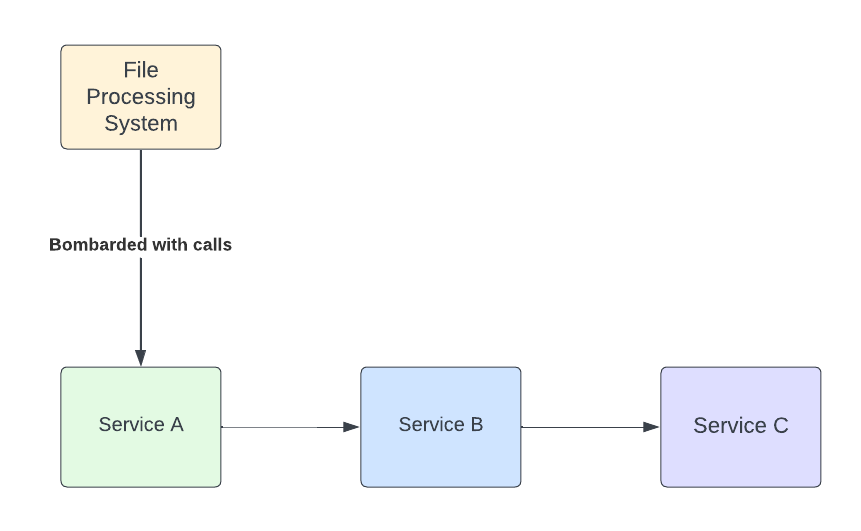
\includegraphics[width=5.5in]{images/initial flow.png}\\[1.5cm]
  \caption{Initial Flow}
  \label{fig:example}
\end{figure}



\section{Knowledge Acquisition}

During the Knowledge Acquisition phase, I focused on acquiring a comprehensive understanding of the domain and technologies relevant to the project. This phase served as the foundation for subsequent development activities, ensuring that I was equipped with the necessary knowledge and skills to execute the project successfully.

\subsection{Understanding the Domain}

The first step of the Knowledge Acquisition phase involved gaining a deep understanding of the domain, specifically the requirements and challenges associated with optimizing the performance and scalability of a high-traffic API system. This included researching common practices, guidelines, and strategies for handling large volumes of requests, mitigating bottlenecks, and ensuring reliable service delivery. The project aimed to improve the efficiency and responsiveness of a backend system dealing with financial transactions.

\subsection{Exploring Technologies}

Simultaneously, I explored the technologies and tools required to implement the desired functionality of the web application. This included a detailed investigation of event-driven architectures, message brokering systems like Kafka, and backend optimization techniques using Java and Spring Boot. Key technologies and tools examined included:

\begin{itemize}
    \item \textbf{Kafka}: Utilized for managing high volumes of requests by separating the request submission from the processing logic, ensuring system responsiveness even under heavy load. In our context, Kafka facilitated the publication of events in the Atropos system, which asynchronously handled the initial flow where the Bill Payments Recon API experienced overwhelming requests.
    
    \item \textbf{Consumer Configuration}: Adjustment of Kafka consumer settings to optimize the simultaneous processing of records, maintaining load balance and preventing system overloads. Configuration adjustments in Atropos, such as `fetch.max.bytes`, `max.poll.records`, and `queued.max.messages.kbytes`, were made to manage the rate of record retrieval and processing effectively.
    
    \item \textbf{Spring Boot}: Employed for developing backend services with efficiency and scalability. In our implementation, Spring Boot facilitated the development of a new API, which, when called by Hades, published events to Kafka topics.
    
    \item \textbf{Grafana}: Utilized for monitoring system metrics, including P99 latency. Grafana enabled the visualization of performance metrics for our APIs, aiding in the identification and resolution of performance bottlenecks.
    
    \item \textbf{Kibana}: Deployed for log management and analysis. Kibana provided insights into log data, enabling effective system monitoring and debugging through visualization of data from Elasticsearch.
    
    \item \textbf{Jenkins}: Employed for continuous integration and deployment to ensure reliable and automated deployment processes. Jenkins facilitated the setup of CI/CD pipelines for automating build, test, and deployment processes, ensuring seamless deployment of system updates.
\end{itemize}

I also evaluated potential integrations and dependencies to ensure compatibility and seamless interaction between different components of the application.

\subsection{Learning Curves and Skill Development}

As part of the Knowledge Acquisition phase, I identified areas where additional learning and skill development were required to effectively contribute to the project. This involved self-study, online courses, tutorials, and hands-on experimentation to gain proficiency in:

\begin{itemize}
    \item \textbf{Backend Development}: This aspect entails enhancing the functionality and efficiency of the backend systems responsible for processing requests. By leveraging Java and Spring Boot, developers focus on writing optimized code that improves system performance and scalability.
    
    \item \textbf{Asynchronous Processing}: Involves the implementation of event-driven architectures, where the processing of requests is decoupled from the submission. By utilizing Kafka, the system can handle requests asynchronously, enhancing responsiveness and scalability.
    
    \item \textbf{Performance Optimization}: Strategies and techniques are employed to fine-tune the performance metrics of the API system. This includes optimizing throughput (the rate at which requests are processed) and latency (the time taken for a request to receive a response), ensuring optimal system performance under varying loads.
    
    \item \textbf{Configuration Management}: This aspect involves understanding and adjusting configurations within the Kafka consumer to manage system loads efficiently. By fine-tuning settings such as the maximum number of records processed simultaneously and the maximum number of requests sent at once, developers can balance loads and optimize system performance.
    
    \item \textbf{Monitoring and Logging}: To ensure system reliability and performance, developers utilize monitoring tools like Grafana to track important metrics such as request rates and response times. Additionally, logging tools like Kibana are employed for effective log management, enabling developers to identify and troubleshoot issues promptly.
    
    \item \textbf{Continuous Integration and Deployment}: Utilizing automation tools like Jenkins, developers streamline the build, testing, and deployment processes. Continuous Integration (CI) ensures that code changes are regularly integrated and tested, while Continuous Deployment (CD) automates the deployment of validated changes to production environments, reducing manual effort and minimizing the risk of errors.
\end{itemize}


By investing time and effort in skill development upfront, I was better equipped to tackle the challenges of the project as it progressed.


\section{Collaboration and Knowledge Sharing}

Regular meetings, brainstorming sessions, and peer reviews were conducted to exchange insights, discuss findings, and address any questions or uncertainties. This collaborative approach fostered a supportive learning environment where we could leverage each other’s expertise and experiences to accelerate our learning curve and collectively drive the project forward.

\subsection{Prototyping and Proof of Concepts}

The Prototyping and Proof of Concept phase is a pivotal step in the development journey, especially when working on complex backend systems. This phase allows for the validation of the technical feasibility and viability of the project’s solution before committing to full-scale development. Let’s delve into the details of how this phase unfolded:

\subsection{Defining Scope and Objectives}

The first task was to clearly define the scope and objectives of the prototype application. This involved identifying the core features and functionalities necessary to achieve the project’s goals. Key components such as API endpoint consolidation, event-driven processing with Kafka, integration with monitoring tools like Grafana and Kibana, and performance optimization were outlined as essential elements to include.

\subsection{Designing Mockups and Wireframes}

With the scope and objectives in mind, the next step was to visualize the user interface and experience of the prototype application. Mockups and wireframes were created using design tools or simple pen and paper to outline the layout, navigation flow, and interaction patterns of key screens and components. These visual representations served as a blueprint for the development process and facilitated communication and alignment throughout the project.

Collaboration and knowledge sharing played a crucial role during this phase. Regular meetings were held to review the progress of the prototype development, brainstorm ideas for improvements, and gather feedback from team members. Peer reviews were conducted to evaluate the effectiveness of the design mockups and wireframes, ensuring that they accurately represented the intended user experience and met the project objectives.

By engaging in collaborative discussions and leveraging the diverse expertise within the team, we were able to refine the scope and objectives of the prototype application, validate its technical feasibility through proof of concepts, and design an intuitive user interface that met the needs of our target audience. This collaborative approach not only accelerated our learning curve but also fostered a sense of ownership and shared responsibility for the success of the project.


\section{Solution}

To address this issue, we redesigned the flow to incorporate asynchronous processing. In the new architecture, the incoming requests are directed to a newly created API. This API then publishes an event to a message broker. Subscriptions within this message broker are configured to handle the asynchronous processing of these events by invoking the existing Service A API.
\\\\
\noindent Previously, there were multiple APIs being called directly. This has been consolidated into a single API that accepts a JSON object as input. Based on an attribute within this JSON object, the event is published to a specific topic. Consumers subscribed to these topics will then call the appropriate existing APIs asynchronously.
\\\\
\noindent To optimize the message broker's configuration and ensure efficient handling of the request load, we made the following adjustments:

\begin{itemize}
    \item \textbf{Max.Tasks.Count}: Defines the number of consumers for a topic. This value is limited by the number of partitions, with the default being one partition and one consumer.
    \item \textbf{Consumer.Override.Max.Poll.Records}: Specifies the number of records a consumer fetches and processes in one poll cycle.
    \item \textbf{Max.Requests.In.Flight}: Determines how many requests a consumer sends out simultaneously, with additional fetched records held in an in-memory buffer.
\end{itemize}

By adjusting these configurations, we were able to balance the load and improve the responsiveness of the system, ensuring that it could handle the increased volume of requests without performance degradation.

\begin{figure}[h]
  \centering
  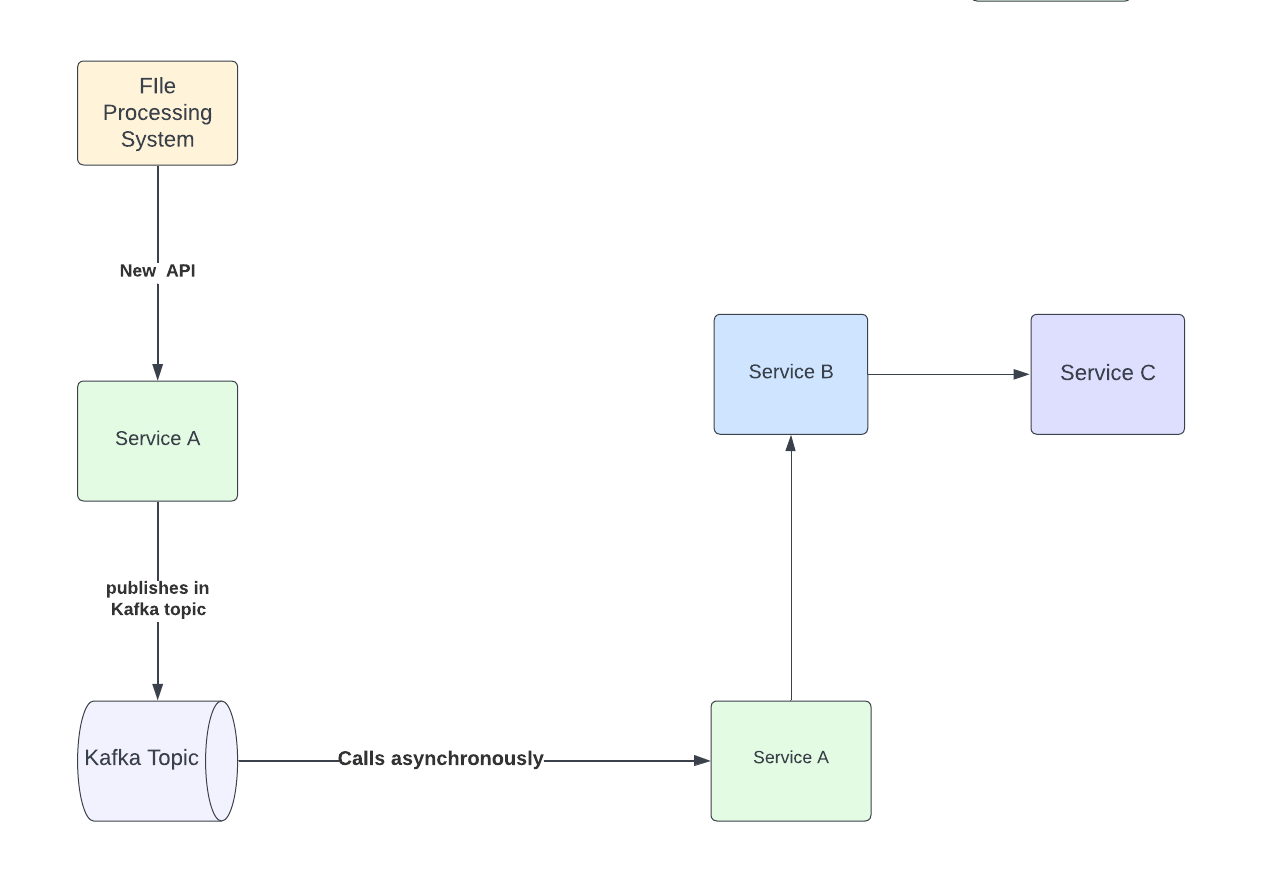
\includegraphics[width=5.5in]{images/final flow1.png}\\[1.5cm]
  \caption{Final Flow}
  \label{fig:example}
\end{figure}


\section{Backend Development}

Backend development serves as the backbone of our system, facilitating the management of business logic, data handling, and communication between the frontend interface and the database. Here's a breakdown of the different aspects of backend development in our project:

\subsection{Setup and Configuration}

The journey into backend development commences with the setup and configuration of our development environment. Leveraging Java as the core programming language and Spring Boot for rapid application development, we initialize the necessary frameworks and tools required for our project. Additionally, we integrate PostgreSQL for robust database solutions and Git for version control to ensure efficient collaboration and code management throughout the development lifecycle.

\subsection{Database Design and Modeling}

A pivotal aspect of backend development involves designing and modeling the database schema. Utilizing Spring Data JPA in conjunction with Hibernate, we define database models using Java entities, abstracting away the complexities of SQL queries. We meticulously design the database schema, considering factors such as data relationships, normalization, and performance optimization. Furthermore, we employ Spring Data JPA's migration system to efficiently manage database schema changes, ensuring seamless data integrity and consistency.

\subsection{API Development}

With the database schema established, we proceed to develop robust APIs (Application Programming Interfaces) to expose functionality to the frontend interface and external clients. Leveraging Spring Boot's powerful REST support, we define RESTful API endpoints for various resources in the application. These endpoints handle incoming HTTP requests, perform data validation, process business logic, and return appropriate HTTP responses in JSON format. Our APIs are meticulously designed to be consistent, predictable, and well-documented, facilitating seamless integration with frontend components and external systems.

\subsection{Business Logic Implementation}

Backend development encompasses the implementation of core business logic, including data processing, validation, and manipulation. Leveraging Java's robust ecosystem and Spring's dependency injection, we write functions and methods to manage user input, enforce business rules, and orchestrate interactions between different components of the system. Our business logic is encapsulated within Spring components, ensuring modularity, reusability, and maintainability of the codebase.

\subsection{Authentication and Authorization}

Security is paramount in backend development, particularly concerning user authentication and authorization. Leveraging Spring Security's comprehensive authentication and authorization mechanisms, we secure our application against unauthorized access and malicious attacks. We configure authentication backends, define user models, and implement access controls to ensure that only authenticated and authorized users can access protected resources. Additionally, we leverage Spring Security's features such as CSRF protection, XSS prevention, and password hashing to mitigate common security vulnerabilities.

\subsection{Testing and Debugging}

Thorough testing and debugging are integral throughout the backend development process to identify and rectify any issues or bugs. We employ JUnit and Mockito for Java testing and Spring's testing framework to develop unit tests, integration tests, and end-to-end tests to validate the functionality and reliability of backend components. Test-driven development (TDD) practices are employed to ensure that code changes undergo comprehensive testing before deployment to production. Additionally, we utilize debugging tools and techniques such as logging, error tracking, and remote debugging to diagnose and resolve issues efficiently, ensuring the stability and performance of the backend system.

\subsection{Deployment and Scalability}

Upon completion of backend development, we prepare for deployment and scalability of the application. We configure deployment environments using Kubernetes for container orchestration and Jenkins for continuous integration and delivery, establishing robust CI/CD pipelines to automate the build, test, and deployment processes. Leveraging AWS for hosting the application, we ensure scalability, reliability, and availability. Additionally, we monitor application performance using Grafana for monitoring and alerting, track usage metrics, and implement scaling strategies such as horizontal scaling or auto-scaling to accommodate increased traffic and workload.

\subsection{File Processing System Configuration}

To efficiently process high volumes of data, we configured our system akin to real-time data streaming solutions like Amazon Kinesis and Apache Flink. This configuration allows for the effective processing of large files by breaking down the data into individual records and processing them asynchronously. The system ensures high throughput and low latency by leveraging Kafka for event streaming, enabling us to process millions of records with robust error handling and retry mechanisms. By adjusting Kafka consumer configurations such as `max.poll.records` and `max.requests.in.flight`, we optimized the balance between load processing and system responsiveness, ensuring smooth and efficient data handling.

\section{Integration and Testing}

Integration and testing play a crucial role in ensuring the reliability, functionality, and performance of our system. In this section, we outline the integration of backend components and the various testing strategies employed to validate our application.

\subsection{Integration of Backend Components}

The integration of backend components involves seamlessly combining individual modules, services, and APIs to form a cohesive system. Leveraging the Spring framework's dependency injection and inversion of control, we integrate backend components such as controllers, services, repositories, and external APIs. In addition to Spring, we also utilize Retrofit, a type-safe HTTP client for Android and Java, for integrating external APIs.
\\\\
\noindent Retrofit simplifies the process of communicating with RESTful APIs by allowing us to define the API endpoints and request parameters as Java interfaces. It handles the conversion of JSON responses to Java objects and provides robust support for error handling and network operations. With Retrofit, we can efficiently consume APIs and incorporate external functionality into our backend system.
\\\\
\noindent By adhering to established design patterns and architectural principles, such as the Model-View-Controller (MVC) pattern and the Repository pattern, we ensure loose coupling and high cohesion between components. This architectural approach facilitates easier maintenance, scalability, and extensibility of our backend system. The use of Retrofit for API integration complements these principles by providing a seamless and efficient mechanism for communicating with external services.

\subsection{Unit Testing}

Unit testing is a fundamental aspect of our testing strategy, focusing on the validation of individual units or components in isolation. Using JUnit and Mockito frameworks for Java testing, we develop unit tests to verify the correctness of methods, functions, and classes within our backend components. By simulating different scenarios and edge cases, we ensure that each unit behaves as expected and adheres to specified requirements. Unit tests are automated and executed frequently during the development process, providing rapid feedback and identifying regressions early in the lifecycle.

\subsection{Integration Testing}

Integration testing is a critical phase in our testing strategy, focusing on evaluating the interactions and dependencies between integrated backend components. It ensures that these components function cohesively as a unified system, providing confidence in the stability and interoperability of the integrated solution.
\\\\
\noindent We leverage the Spring framework's testing capabilities, specifically the MockMVC module, for integration testing. MockMVC allows us to simulate HTTP requests and responses, enabling comprehensive testing of controllers and their interactions with other components. Additionally, we utilize the REST Assured library, which provides a fluent API for testing RESTful APIs, to validate the communication between our backend services and external dependencies.
\\\\
\noindent Our integration tests encompass a wide range of scenarios, including end-to-end user journeys, error handling, and data flow validation. By simulating API requests and responses, we verify the correctness of data transmission, authentication mechanisms, and response formats. This ensures that our system behaves as expected under various conditions and gracefully handles errors and edge cases.
\\\\
\noindent In summary, integration testing plays a crucial role in validating the interoperability and functionality of our integrated backend components. By leveraging MockMVC and REST Assured, we can comprehensively test the communication between components and ensure the reliability and robustness of our system.


\subsection{Performance Testing}

Performance testing is essential for evaluating system responsiveness, scalability, and resource utilization, particularly in handling individual records from uploaded files and making API calls for each record. Our approach, resembling real-time data streaming systems like Amazon Kinesis or Apache Flink, focuses on measuring the latency of processing individual records, especially the 99th percentile (P99) requests. This metric provides insight into typical latency, helping us understand system performance under normal conditions.
\\\\
\noindent To conduct performance testing, we simulate file uploads with varying record counts and measure the time taken to process each record. We employ real-time monitoring and logging to capture and analyze API call latency for individual record processing. By adjusting the load and observing system response, we identify performance bottlenecks, scalability constraints, or areas needing optimization.

Our performance testing strategy includes the following key components:

\begin{itemize}
    \item \textbf{Request Per Second (RPS) Measurement}: We track the number of requests processed by the system per second. This metric helps us understand the system's throughput and its ability to handle concurrent requests. By increasing the number of simulated file uploads and monitoring RPS, we can determine the system's maximum capacity and identify any throughput limitations.

    \item \textbf{Latency Analysis}: In addition to measuring the average latency, we focus on the P99 latency, which represents the time within which 99% of the requests are processed. This provides a more comprehensive view of the system's performance, highlighting any outliers that may affect the user experience. We also monitor other latency percentiles (e.g., P90, P95) to gain a broader understanding of system performance.

    \item \textbf{Resource Utilization Monitoring}: We continuously monitor system resources such as CPU, memory, and disk usage during performance testing. This helps us identify any resource bottlenecks that may impact the system's ability to handle high loads. By correlating resource utilization with performance metrics, we can pinpoint areas that require optimization.

    \item \textbf{Scalability Testing}: We evaluate the system's ability to scale horizontally and vertically by adding more processing nodes or increasing the capacity of existing nodes. This involves testing the system under varying loads to ensure it can handle increased traffic without degradation in performance.

    \item \textbf{Error Rate Tracking}: Monitoring the error rate during performance testing is crucial for identifying issues related to request handling. We track the number of failed requests and analyze the root causes to improve system reliability and robustness.

    \item \textbf{Real-Time Monitoring and Logging}: Utilizing tools such as Grafana and Kibana, we set up dashboards to visualize key performance metrics in real-time. This allows us to quickly identify and address performance issues as they arise. Detailed logs help us trace the flow of individual requests and diagnose problems effectively.

    \item \textbf{Iterative Optimization}: Performance testing is an ongoing process conducted throughout the development lifecycle. By iteratively testing and optimizing the system, we ensure that it meets the required performance criteria and can handle expected user traffic. This approach allows us to make incremental improvements and validate them against real-world scenarios.
\end{itemize}

Our iterative performance testing process occurs throughout development and before production deployment, ensuring the system meets performance criteria and can handle expected user traffic. Focusing on individual record processing latency, request per second, and other key performance metrics provides valuable insights for optimizing system performance and enhancing the user experience. This comprehensive approach ensures that our web application is robust, scalable, and capable of delivering a high-quality user experience even under heavy load conditions.



\subsection{User Acceptance Testing (UAT)}

\subsubsection{Overview}

User Acceptance Testing (UAT) is a critical phase in the software development lifecycle, designed to verify the application's functionality, usability, and alignment with user requirements by conducting real-world testing with end-users or stakeholders. This phase ensures that the application meets the business objectives and user expectations before it is deployed to the production environment.

\subsubsection{UAT Environment}

In our company, UAT is conducted in a dedicated zone or environment that closely mimics the production environment. This UAT environment is configured to replicate production settings as accurately as possible, ensuring that any issues identified during testing are likely to manifest in the production environment as well. This environment includes the same server configurations, database settings, and network conditions to provide a realistic testing ground for the application.

\subsubsection{UAT Process}

The UAT process involves several key steps to ensure thorough testing and validation:

\begin{itemize}
    \item \textbf{Collaborative Planning:} We collaborate closely with stakeholders to outline test scenarios, acceptance criteria, and user stories tailored for UAT. This collaborative approach ensures that the testing is aligned with user expectations and business requirements.
    
    \item \textbf{Manual Testing:} Testers engage in manual testing to evaluate the application's features, workflows, and user interfaces. They follow the predefined test scenarios and acceptance criteria to systematically test the application, focusing on functionality, usability, and overall user experience.
    
    \item \textbf{Feedback and Issue Tracking:} Testers provide valuable feedback on usability, accessibility, and any encountered issues. All feedback and identified issues are meticulously documented and tracked using issue tracking tools. This feedback is critical for identifying areas of improvement and ensuring that the application meets user expectations.
    
    \item \textbf{Issue Resolution:} The development team addresses the identified issues and incorporates the feedback into the application. This iterative process of testing, feedback, and issue resolution continues until the application is deemed ready for final deployment.
    
    \item \textbf{Final Review and Approval:} Once all identified issues have been resolved and the application has been refined based on user feedback, a final review is conducted. Stakeholders review the application to ensure that it aligns with the outlined acceptance criteria and business objectives. Upon approval, the application is prepared for production deployment.
\end{itemize}

\subsubsection{UAT Application}

For specific applications like the PayZapp app, UAT plays a crucial role in ensuring seamless functionality and user experience. The UAT environment for PayZapp is set up to simulate real-world usage scenarios as closely as possible. Any changes or updates to the PayZapp app are first deployed to the UAT environment where comprehensive testing is conducted. This includes:

\begin{itemize}
    \item \textbf{Transaction Testing:} Verifying that all transaction-related functionalities work correctly, including payment processing, refunds, and transaction history.
    
    \item \textbf{Security Testing:} Ensuring that security features such as encryption, authentication, and authorization are functioning correctly to protect user data.
    
    \item \textbf{Performance Testing:} Assessing the app's performance under various conditions to ensure it can handle expected user loads without degradation in performance.
    
    \item \textbf{User Interface Testing:} Checking that the user interface is intuitive and user-friendly, and that all elements are displayed correctly on different devices and screen sizes.
    
    \item \textbf{Integration Testing:} Ensuring that the app integrates seamlessly with other systems and services, such as banking APIs, third-party payment gateways, and notification services.
\end{itemize}

The results of UAT for the PayZapp app are meticulously reviewed, and any identified issues are addressed promptly. This ensures that when changes are eventually deployed to production, they are robust, secure, and provide a seamless user experience.

By conducting thorough UAT, we ensure that our applications not only meet the technical requirements but also deliver a superior user experience, ultimately enhancing user satisfaction and achieving business goals.

\section{Deployment and Documentation}

Deployment and documentation are critical phases in the development lifecycle, ensuring that the web application is successfully deployed to production environments and that comprehensive documentation is provided to support its usage, maintenance, and future development.


\subsection{Deployment Process}

The deployment process involves preparing the web application for release and deploying it to production environments where it can be accessed by users. This process typically includes the following steps:

\begin{itemize}
    \item \textbf{Environment Configuration:} Configure production environments, including servers, databases, and networking infrastructure, to host the web application. Set up security measures such as firewalls, SSL certificates, and access controls to protect sensitive data and ensure compliance with security standards.
    
    \item \textbf{Build and Packaging:} Package the application code, assets, and dependencies into deployable artifacts such as Docker containers or deployment packages. Perform build optimizations and asset minification to improve performance and reduce load times.
    
    \item \textbf{Continuous Integration and Deployment (CI/CD):} Set up CI/CD pipelines to automate the build, test, and deployment processes. Utilize tools such as Jenkins, GitLab CI/CD, or GitHub Actions to trigger automated builds, run tests, and deploy updates to production environments seamlessly.
    
    \item \textbf{Deployment Strategy:} Choose an appropriate deployment strategy such as blue-green deployments, canary deployments, or rolling updates to minimize downtime and ensure zero-downtime deployments. Monitor deployment progress and rollback changes if necessary to mitigate any issues or errors.

    \item \textbf{Change Management:} Before initiating the deployment, create a change management ticket to document the proposed changes, including the scope, impact, and rollback plan. Obtain necessary approvals from stakeholders and change management boards to ensure that the deployment aligns with organizational policies and procedures.

    \item \textbf{Tagging and Deployment:} Build the application and create a version tag to uniquely identify the release. Collaborate with Site Reliability Engineers (SREs) to deploy the tagged version to the production environment, ensuring that deployment processes follow best practices and organizational standards.

    \item \textbf{Service Synchronization:} Ensure that the service synchronization process is in place to align the new deployment with existing services. This includes updating service discovery mechanisms, reconfiguring load balancers, and validating that all dependent services are correctly synchronized with the new deployment.

\end{itemize}

\subsection{Documentation}

Comprehensive documentation is essential for guiding users, administrators, and developers in understanding and utilizing the web application effectively. Documentation should cover various aspects of the application, including its architecture, functionality, usage, configuration, and troubleshooting. Key components of documentation include:

\begin{itemize}
    \item \textbf{Installation Guide:} Provide step-by-step instructions for installing and configuring the web application in different environments, including development, staging, and production. Include prerequisites, dependencies, and configuration settings required for successful installation.
    
    \item \textbf{User Manual:} Create user manuals or user guides that explain how to use the web application's features and functionalities. Include screenshots, examples, and best practices to help users navigate the application and accomplish common tasks.
    
    \item \textbf{Administrator Guide:} Document administrative tasks such as user management, configuration settings, and system maintenance procedures. Provide guidance on managing user accounts, monitoring system health, and troubleshooting common issues.
    
    \item \textbf{API Documentation:} If the web application exposes APIs for integration with external systems, provide comprehensive API documentation that describes endpoints, request/response formats, authentication mechanisms, and usage examples. Use tools such as Swagger or OpenAPI to generate interactive API documentation.
    
    \item \textbf{Release Notes:} Maintain release notes or changelogs that document changes, enhancements, and bug fixes introduced in each version of the web application. Include information about new features, improvements, and any breaking changes that may affect users or developers.
    
    \item \textbf{Troubleshooting Guide:} Compile a troubleshooting guide that outlines common issues, error messages, and resolutions encountered when using the web application. Provide troubleshooting steps, diagnostic tools, and recommended solutions for resolving problems efficiently.

    \item \textbf{Lucidchart Diagrams:} Utilize Lucidchart to create visual diagrams representing the application's architecture, data flow, and process workflows. These diagrams aid in understanding complex structures and interactions within the system, providing a clear visual representation of how different components are interconnected.

    \item \textbf{Swimlane Diagrams:} Develop swimlane diagrams to map out processes, tasks, and responsibilities across different actors or components in the system. These diagrams help clarify the sequence of operations and the roles of various elements, enhancing clarity and ensuring efficient process management.

\end{itemize}

\section{Bug Fixes}

Bug fixes are an integral part of the software development lifecycle, ensuring that issues and defects identified during testing or after deployment are addressed promptly and effectively. In this phase, we focus on identifying, prioritizing, and resolving bugs to improve the reliability, performance, and user experience of the web application.

\subsection{Bug Identification and Prioritization}

The bug fixing process begins with identifying and documenting bugs reported by users, testers, or detected through automated testing processes. Bugs may manifest as functional issues, performance bottlenecks, security vulnerabilities, or compatibility problems across different platforms or devices. Once identified, bugs are triaged and prioritized based on their severity, impact on user experience, and business impact. Critical bugs that affect core functionality or security are prioritized for immediate resolution, while minor bugs may be scheduled for future releases or addressed as part of regular maintenance cycles.

\subsection{Root Cause Analysis}

Once bugs are prioritized, the next step is to perform root cause analysis to understand the underlying reasons for their occurrence. This involves investigating the source code, reviewing logs and error messages, and reproducing the issue in a controlled environment. By identifying the root cause of bugs, we gain insights into the factors contributing to their occurrence and can implement effective solutions to prevent similar issues from reoccurring in the future.

\subsection{Fix Implementation}

After identifying the root cause, fixes are implemented to address the bugs. This may involve modifying source code, updating configurations, or applying patches to third-party dependencies. Care is taken to ensure that fixes are implemented correctly and do not introduce new issues or regressions in the application.

\subsection{Testing and Validation}

Once fixes are implemented, comprehensive testing is conducted to validate their effectiveness and verify that the bugs have been resolved satisfactorily. Unit tests, integration tests, and regression tests are executed to ensure that the fixes do not introduce new issues or regressions in the application. Test cases are designed to cover the specific scenarios and conditions associated with each bug, ensuring that fixes are verified under relevant use cases and edge cases. User acceptance testing may also be conducted to validate fixes from a user perspective and ensure that they meet user expectations and requirements.

\subsection{Release and Monitoring}

Once fixes are validated, they are incorporated into the next release of the web application. Release notes or changelogs are updated to document the fixes included in the release, providing transparency and accountability to users and stakeholders. After release, ongoing monitoring and feedback mechanisms are established to track the effectiveness of fixes in production environments and identify any new issues or regressions that may arise. Continuous monitoring allows for proactive detection and resolution of issues, ensuring the stability and reliability of the web application over time.

\chapter{Conclusion}

\noindent This project successfully addressed the challenges of developing and optimizing a high-traffic API system for financial transactions. By leveraging comprehensive knowledge acquisition and targeted skill development, we established a solid foundation for the backend architecture, integrating robust technologies such as Kafka, Spring Boot, and Jenkins. This approach not only facilitated the handling of large volumes of requests but also ensured system responsiveness and reliability, crucial for financial applications.
\\\\
\noindent The implementation phase underscored the importance of meticulous backend development, including database design, API creation, and business logic integration. Through rigorous testing strategies—spanning unit, integration, performance, and user acceptance testing—we validated the system’s functionality and performance, ensuring it met stringent quality standards. Security measures were rigorously applied to protect sensitive financial data, reinforcing the system’s reliability and user trust.
\\\\
\noindent The deployment process, supported by CI/CD pipelines and Kubernetes, ensured seamless and scalable production releases. Comprehensive documentation provided a vital resource for users and administrators, enhancing the system’s usability and maintainability. The iterative approach to bug fixing and continuous monitoring highlighted our commitment to long-term stability and performance. This project exemplifies a holistic and collaborative methodology in developing high-traffic API systems, setting a benchmark for future projects in similar domains.


 
\begin{thebibliography}{9}
\addcontentsline{toc}{chapter}{BIBLIOGRAPHY}
\bibitem{java}
Oracle. (2023). Java Platform, Standard Edition Documentation. Available at: \url{https://docs.oracle.com/en/java/}

\bibitem{spring}
Pivotal Software, Inc. (2023). Spring Framework Documentation. Available at: \url{https://spring.io/projects/spring-framework}

\bibitem{springboot}
Pivotal Software, Inc. (2023). Spring Boot Reference Guide. Available at: \url{https://docs.spring.io/spring-boot/docs/current/reference/htmlsingle/}

\bibitem{postgresql}
PostgreSQL Global Development Group. (2023). PostgreSQL 14 Documentation. Available at: \url{https://www.postgresql.org/docs/14/}

\bibitem{kafka}
Apache Software Foundation. (2023). Apache Kafka Documentation. Available at: \url{https://kafka.apache.org/documentation/}

\bibitem{jenkins}
Jenkins Project. (2023). Jenkins User Documentation. Available at: \url{https://www.jenkins.io/doc/}

\bibitem{grafana}
Grafana Labs. (2023). Grafana Documentation. Available at: \url{https://grafana.com/docs/}

\bibitem{kibana}
Elastic. (2023). Kibana Guide [7.15]. Available at: \url{https://www.elastic.co/guide/en/kibana/current/index.html}

\bibitem{aws}
Amazon Web Services, Inc. (2023). AWS Documentation. Available at: \url{https://docs.aws.amazon.com/}

\bibitem{flink}
Apache Software Foundation. (2023). Apache Flink Documentation. Available at: \url{https://flink.apache.org/documentation.html}

\bibitem{kinesis}
Amazon Web Services, Inc. (2023). Amazon Kinesis Documentation. Available at: \url{https://docs.aws.amazon.com/kinesis/}

\end{thebibliography}

\end{document}

% Add your references here
\end{document}
